\documentclass[11pt]{article}

% ── Packages ────────────────────────────────────────────────────────────────
\usepackage[margin=1in]{geometry}
\usepackage{amsmath, amssymb, amsthm}
\usepackage{graphicx}
\usepackage{booktabs}
\usepackage{caption}
\usepackage{subcaption}
\usepackage{hyperref}
\usepackage{xcolor}
\usepackage{setspace}

\hypersetup{
  colorlinks=true,
  linkcolor=blue!60!black,
  citecolor=blue!60!black,
  urlcolor=blue!60!black
}

% ── Title ────────────────────────────────────────────────────────────────────
\title{%
  \textbf{Numerical Interpolation Study on Housing Price Data}\\[4pt]
  \large CMPSC 456 --- Track A Project Report
}
\author{Peidong Liu}
\date{March 2026}

% ─────────────────────────────────────────────────────────────────────────────
\begin{document}
\maketitle
\tableofcontents
\newpage

% =============================================================================
\section{Problem Statement and Project Goals}
% =============================================================================

Housing prices are influenced by a complex combination of physical attributes
(floor area, number of bedrooms and bathrooms, stories), locational factors
(proximity to main road, preferred area), and amenity features (air
conditioning, hot water heating, furnishing status).  Following a period of
significant market volatility, accurately modeling the relationship between
these features and transaction prices is of both practical and theoretical
interest.

From a numerical analysis perspective, housing data presents a natural
testbed for interpolation methods: the price--area curve is non-trivial,
exhibits local variability, and is defined only at discrete sample points,
mirroring the classical setting in which polynomial and spline approximation
theory was developed.

\subsection*{Goals}

This project pursues three interconnected goals:

\begin{enumerate}
  \item \textbf{Compare node distributions.}  Quantify the difference in
        accuracy and stability between \emph{equispaced} and \emph{Chebyshev}
        nodes for barycentric polynomial interpolation of price--area data.

  \item \textbf{Demonstrate Runge-type behavior.}  Show empirically that the
        $L^\infty$ interpolation error with equispaced nodes diverges as
        polynomial degree increases, while Chebyshev nodes remain stable.

  \item \textbf{Evaluate cubic spline boundary conditions.}  Compare three
        standard boundary conditions --- natural, clamped, and
        not-a-knot --- in terms of accuracy ($L^2$ and $L^\infty$ norms) and
        qualitative smoothness.
\end{enumerate}

% =============================================================================
\section{Dataset and Feature Engineering}
% =============================================================================

\subsection{Dataset}

The dataset is the \emph{Housing Price Data} published on Kaggle by
Saurabhbadole, containing $n = 545$ residential property transactions with
13 attributes: \texttt{price}, \texttt{area}, \texttt{bedrooms},
\texttt{bathrooms}, \texttt{stories}, \texttt{mainroad}, \texttt{guestroom},
\texttt{basement}, \texttt{hotwaterheating}, \texttt{airconditioning},
\texttt{parking}, \texttt{prefarea}, and \texttt{furnishingstatus}.
Prices range from \$1{,}750{,}000 to \$13{,}300{,}000; floor areas range
from 1{,}650 to 16{,}200 sq.\,ft.

\subsection{Feature Selection and Preprocessing}

For a univariate interpolation study the most interpretable single predictor
is \textbf{area} (floor area in sq.\,ft.), which captures the dominant driver
of price in standard hedonic pricing models.

Preprocessing steps:
\begin{enumerate}
  \item All six binary categorical columns (\texttt{mainroad},
        \texttt{guestroom}, \texttt{basement}, \texttt{hotwaterheating},
        \texttt{airconditioning}, \texttt{prefarea}) were encoded as $0/1$
        integers.
  \item \texttt{furnishingstatus} was mapped to an ordinal scale
        (\texttt{unfurnished}$=0$, \texttt{semi-furnished}$=1$,
        \texttt{furnished}$=2$).
  \item Records were sorted by area in ascending order.
  \item A subsample of $m = 60$ evenly-indexed rows was extracted to keep the
        interpolation problem tractable and reduce the influence of outliers.
  \item Both \texttt{area} and \texttt{price} were linearly normalized to the
        canonical interval $[-1,\,1]$ via
        \[
          \tilde{x} = \frac{2(x - x_{\min})}{x_{\max} - x_{\min}} - 1,
          \qquad
          \tilde{y} = \frac{2(y - y_{\min})}{y_{\max} - y_{\min}} - 1,
        \]
        so that all interpolation methods operate on the same domain and
        numerical magnitudes are comparable.
\end{enumerate}

Normalization to $[-1,1]$ is standard practice: it maps Chebyshev node
formulas directly to the data domain and avoids large condition numbers caused
by widely differing coordinate scales.

% =============================================================================
\section{Numerical Methods}
% =============================================================================

\subsection{Barycentric Polynomial Interpolation}

Given $n$ distinct nodes $x_1 < x_2 < \cdots < x_n$ in $[-1,1]$ with
function values $y_k = f(x_k)$, the unique interpolating polynomial of degree
at most $n-1$ can be written in \emph{barycentric form}:

\begin{equation}
  p(x) = \frac{\displaystyle\sum_{k=1}^{n} \frac{w_k}{x - x_k}\,y_k}
              {\displaystyle\sum_{k=1}^{n} \frac{w_k}{x - x_k}},
  \label{eq:bary}
\end{equation}

where the \emph{barycentric weights} are
\[
  w_k = \frac{1}{\prod_{j \neq k}(x_k - x_j)}.
\]

The barycentric form is preferred over the Newton or Lagrange forms for two
reasons: (1) it requires only $O(n)$ operations per evaluation once the
weights are precomputed, and (2) it is backward stable --- small perturbations
in the weights produce proportionally small perturbations in $p(x)$
\cite{higham2004}.

\subsection{Equispaced Nodes}

Equispaced nodes on $[-1,1]$ are defined by
\[
  x_k^{\mathrm{eq}} = -1 + \frac{2(k-1)}{n-1}, \quad k = 1, \ldots, n.
\]

The Lebesgue constant for equispaced nodes grows exponentially as
$\Lambda_n \sim \frac{2^n}{en\ln n}$, making interpolation increasingly
sensitive to perturbations in $y_k$ as $n$ grows.

\subsection{Chebyshev Nodes (First Kind)}

The $n$ Chebyshev nodes of the first kind on $[-1,1]$ are
\[
  x_k^{\mathrm{cheb}} = \cos\!\left(\frac{(2k-1)\pi}{2n}\right),
  \quad k = 1, \ldots, n.
\]

These nodes are the zeros of the Chebyshev polynomial $T_n(x)$.  They are
densest near the endpoints $\pm 1$, which counteracts the Runge phenomenon.
The Lebesgue constant for Chebyshev nodes grows only logarithmically,
$\Lambda_n \sim \frac{2}{\pi}\ln n + O(1)$, giving uniformly bounded
interpolation error for smooth functions.

\subsection{Runge Phenomenon}

The \emph{Runge phenomenon} describes the failure of high-degree polynomial
interpolation at equispaced nodes: for many smooth functions the $L^\infty$
interpolation error \emph{increases} with $n$ instead of decreasing.  The
classical example is $f(x) = 1/(1+25x^2)$.  The underlying cause is that the
norm of the interpolation operator (the Lebesgue constant) grows faster than
the best polynomial approximation error shrinks.

\subsection{Cubic Spline Interpolation}

A \emph{cubic spline} $S(x)$ is a piecewise-cubic function on $[x_1, x_n]$
that satisfies:
\begin{itemize}
  \item $S(x_k) = y_k$ for all $k$ (interpolation conditions),
  \item $S$, $S'$, and $S''$ are continuous on $[x_1, x_n]$.
\end{itemize}

This leaves two degrees of freedom, which are fixed by the boundary conditions:

\begin{description}
  \item[Natural:] $S''(x_1) = S''(x_n) = 0$.  Minimizes the integrated
        squared curvature $\int (S'')^2\,dx$.
  \item[Clamped:] $S'(x_1) = S'(x_n) = 0$.  Prescribes zero first derivative
        at the endpoints; appropriate when the slope is known to flatten.
  \item[Not-a-Knot:] The third derivative $S'''$ is continuous across the
        second knot $x_2$ and the second-to-last knot $x_{n-1}$.  This
        condition is used in MATLAB's \texttt{spline} function and IMSL
        libraries.
\end{description}

\subsection{Error Norms}

Two error norms are used throughout:
\[
  \|e\|_\infty = \max_{i}\,|p(x_i) - f(x_i)|
  \quad \text{(worst-case / minimax error)},
\]
\[
  \|e\|_2 = \sqrt{\frac{1}{N}\sum_{i=1}^{N}|p(x_i) - f(x_i)|^2}
  \quad \text{(RMS error)},
\]

where $\{x_i\}_{i=1}^{N}$ is a dense evaluation grid of $N = 500$ points.
The $L^\infty$ norm captures the \emph{maximum pointwise deviation} and is
most sensitive to localized oscillations, while the $L^2$ norm captures
\emph{average accuracy} and is less influenced by isolated spikes.

% =============================================================================
\section{Results}
% =============================================================================

\subsection{Experiment 1: Equispaced vs.\ Chebyshev at $n = 15$}

\begin{figure}[h]
  \centering
  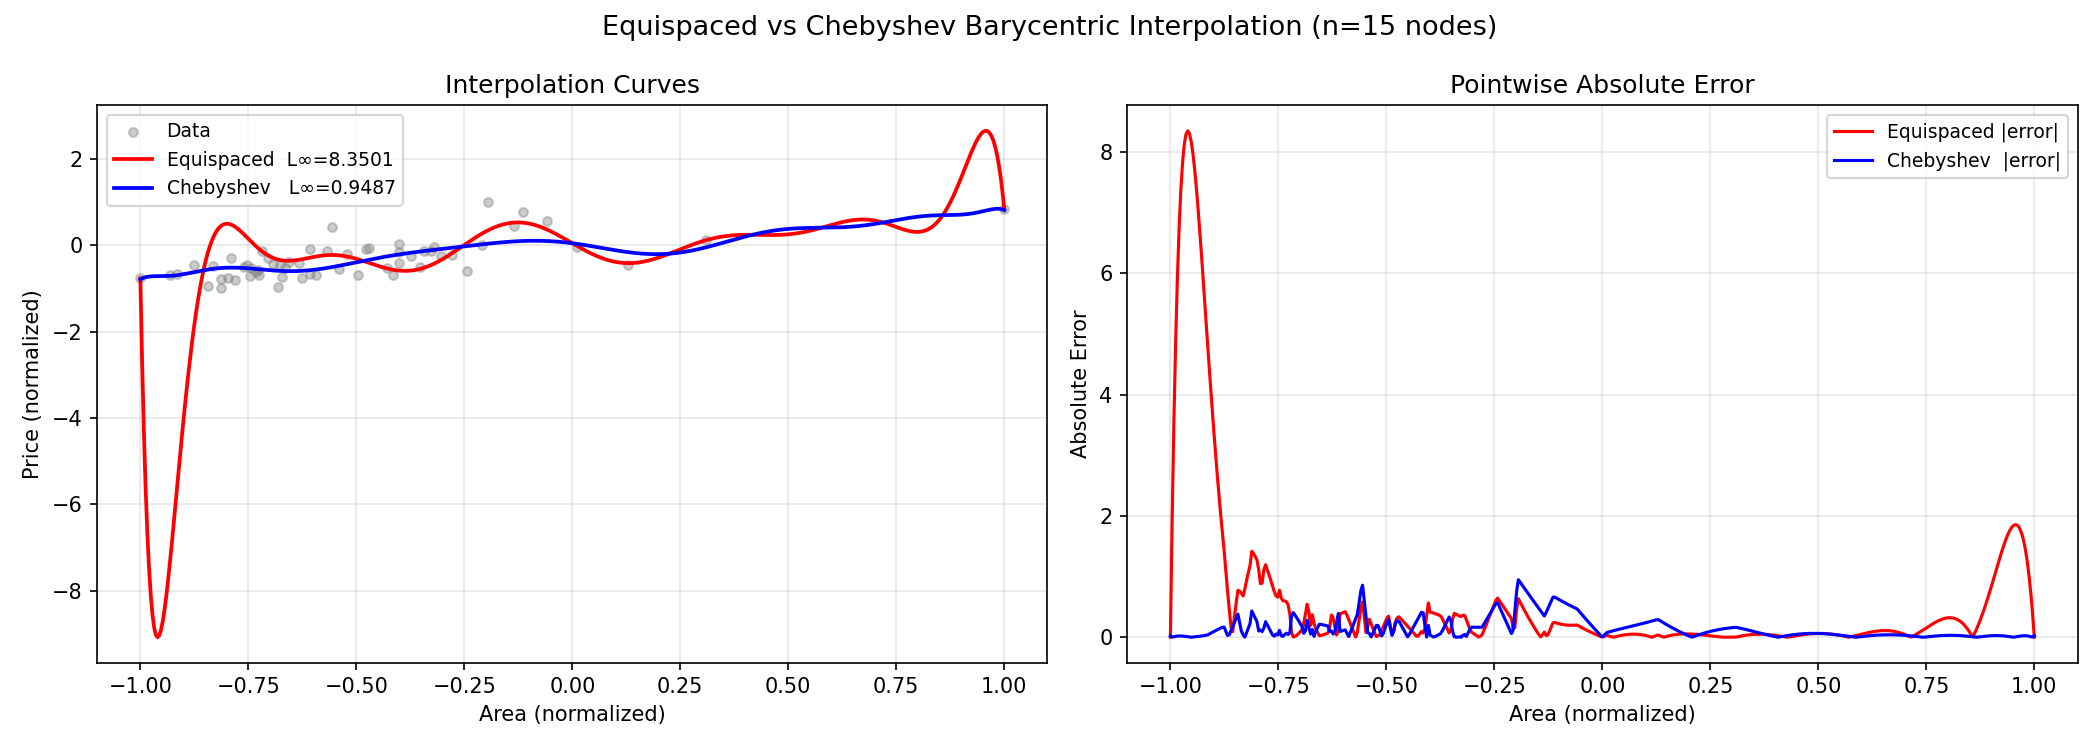
\includegraphics[width=\linewidth]{plot1_equi_vs_cheb.png}
  \caption{%
    \textbf{Left:} Barycentric interpolating polynomials through $n=15$ nodes
    for equispaced (red) and Chebyshev (blue) distributions.  The data
    subsample is shown as gray points.
    \textbf{Right:} Corresponding pointwise absolute errors over the
    evaluation grid.  The equispaced curve exhibits a large spike near
    $x \approx -0.95$ (the left boundary), while Chebyshev errors are
    uniformly small.
  }
  \label{fig:equi_vs_cheb}
\end{figure}

\begin{table}[h]
  \centering
  \caption{Error comparison at $n = 15$ nodes (normalized scale).}
  \label{tab:equi_vs_cheb}
  \begin{tabular}{lcc}
    \toprule
    Method & $L^\infty$ Error & $L^2$ (RMS) Error \\
    \midrule
    Equispaced (barycentric) & 8.3501 & 1.5317 \\
    Chebyshev  (barycentric) & 0.9487 & 0.2316 \\
    \bottomrule
  \end{tabular}
\end{table}

At $n=15$ nodes, Chebyshev interpolation achieves a factor of $\mathbf{8.8\times}$
reduction in $L^\infty$ error and a factor of $\mathbf{6.6\times}$ reduction
in $L^2$ error relative to equispaced nodes (Table~\ref{tab:equi_vs_cheb}).
The error plot (Figure~\ref{fig:equi_vs_cheb}, right) makes the source of
the discrepancy clear: the equispaced polynomial produces a large, localized
oscillation at the left boundary ($x \approx -1$) where the node density
relative to the rate of variation in the data is lowest.  The Chebyshev
polynomial's error is distributed more uniformly and remains below $1$ across
the entire domain.

\subsection{Experiment 2: Runge-Type Oscillation Across Degrees}

\begin{figure}[h]
  \centering
  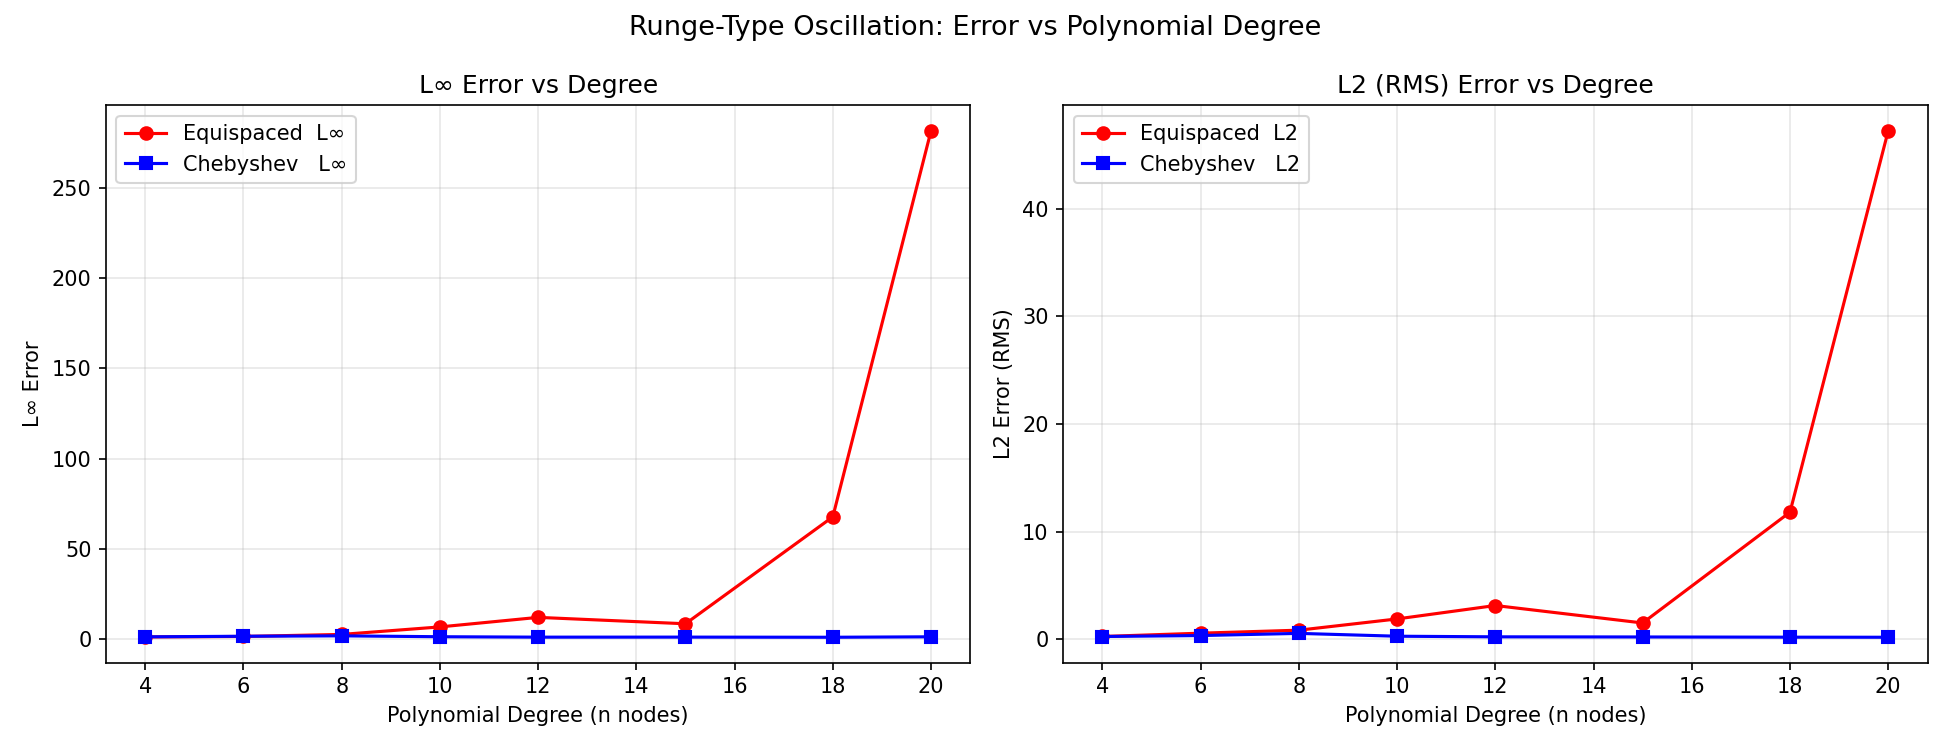
\includegraphics[width=\linewidth]{plot2_runge_analysis.png}
  \caption{%
    $L^\infty$ (left) and $L^2$ RMS (right) interpolation errors as
    polynomial degree increases from 4 to 20 nodes.  Equispaced errors
    (red) exhibit exponential growth; Chebyshev errors (blue) remain
    near or below 1 throughout.
  }
  \label{fig:runge_analysis}
\end{figure}

\begin{table}[h]
  \centering
  \caption{%
    $L^\infty$ and $L^2$ (RMS) errors as a function of the number of
    interpolation nodes $n$.  All errors are in normalized units.
  }
  \label{tab:runge}
  \begin{tabular}{ccccc}
    \toprule
    $n$ & Equispaced $L^\infty$ & Chebyshev $L^\infty$ & Equispaced $L^2$ & Chebyshev $L^2$ \\
    \midrule
     4  &   1.051 &  1.100 &  0.277 & 0.276 \\
     6  &   1.314 &  1.425 &  0.585 & 0.364 \\
     8  &   2.445 &  1.654 &  0.863 & 0.565 \\
    10  &   6.606 &  1.163 &  1.907 & 0.301 \\
    12  &  11.896 &  0.925 &  3.153 & 0.246 \\
    15  &   8.350 &  0.949 &  1.532 & 0.232 \\
    18  &  67.640 &  0.868 & 11.820 & 0.213 \\
    20  & 281.726 &  1.119 & 47.231 & 0.205 \\
    \bottomrule
  \end{tabular}
\end{table}

\begin{figure}[h]
  \centering
  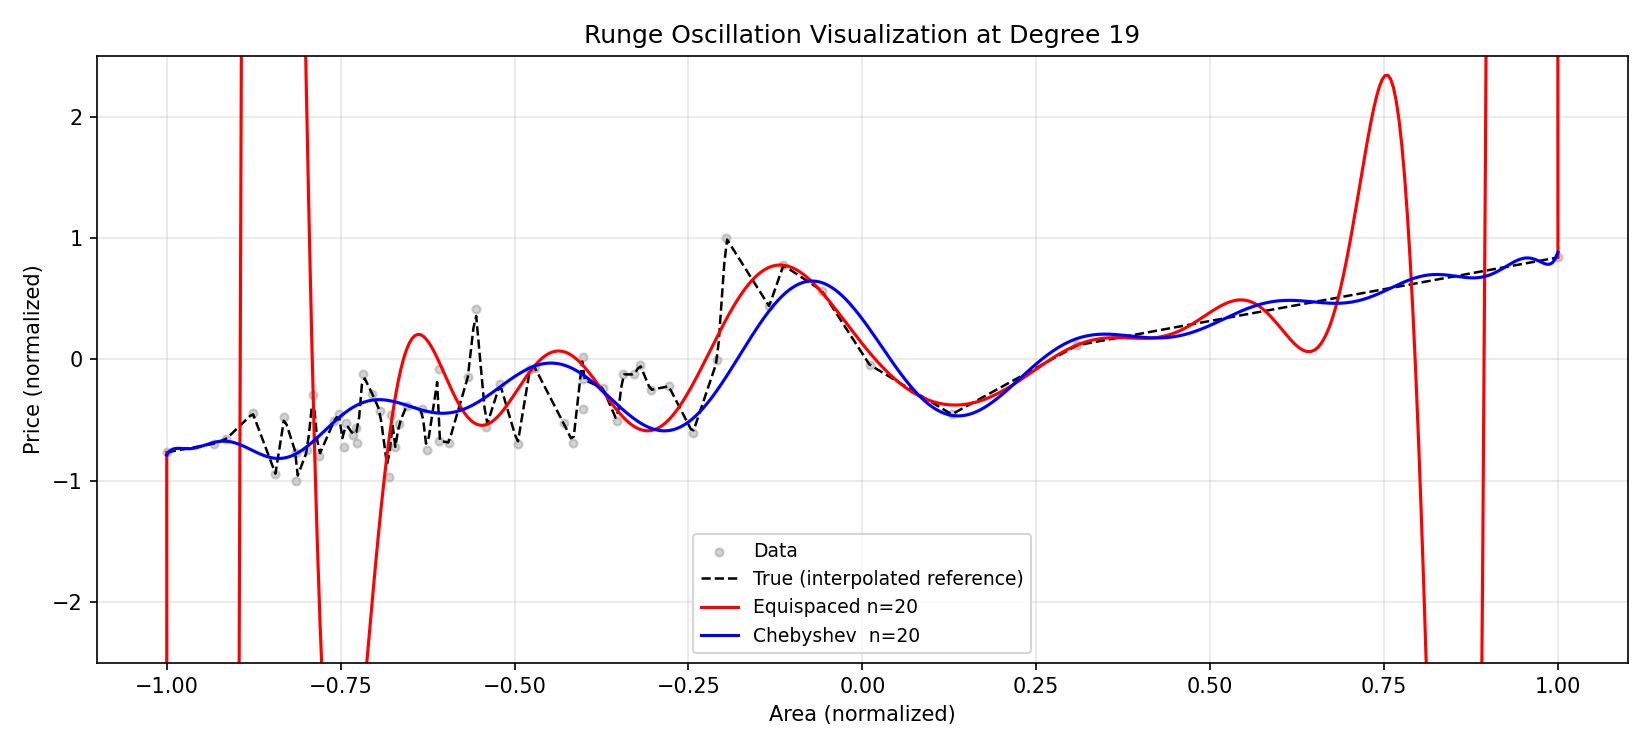
\includegraphics[width=\linewidth]{plot3_runge_visual.png}
  \caption{%
    Runge oscillation visualization at degree 19 ($n = 20$).  The equispaced
    polynomial (red) diverges with spikes exceeding $|\tilde{y}| = 2.5$
    at multiple locations, particularly near the endpoints.
    The Chebyshev polynomial (blue) closely tracks the reference curve
    (dashed black) throughout the domain.
  }
  \label{fig:runge_visual}
\end{figure}

The Runge-type instability of equispaced interpolation is strikingly
demonstrated in Table~\ref{tab:runge} and Figures~\ref{fig:runge_analysis}
and \ref{fig:runge_visual}.  At low degrees ($n \leq 6$) both methods perform
comparably.  Above $n = 8$, equispaced $L^\infty$ error begins to grow
rapidly, reaching $281.7$ at $n = 20$ --- a value $\mathbf{252\times}$ larger
than the corresponding Chebyshev error of $1.12$.

Chebyshev $L^\infty$ errors, by contrast, oscillate mildly between $0.87$
and $1.1$ and show no systematic growth, consistent with the theoretical
bound:
\[
  \|f - p_n^{\mathrm{cheb}}\|_\infty \leq
  \frac{\|f^{(n+1)}\|_\infty}{2^n(n+1)!}\cdot\frac{1}{2^n},
\]
which decreases with $n$ for smooth $f$.  The non-monotone behavior visible
at small $n$ reflects genuine irregularity in the housing data rather than
a theoretical violation.

Figure~\ref{fig:runge_visual} provides an interpretable visual account: at
$n=20$ the equispaced polynomial produces unphysical spikes that vastly exceed
the range of normalized prices, while the Chebyshev polynomial remains a
plausible smooth fit to the data.

\subsection{Experiment 3: Cubic Spline Boundary Conditions}

\begin{figure}[h]
  \centering
  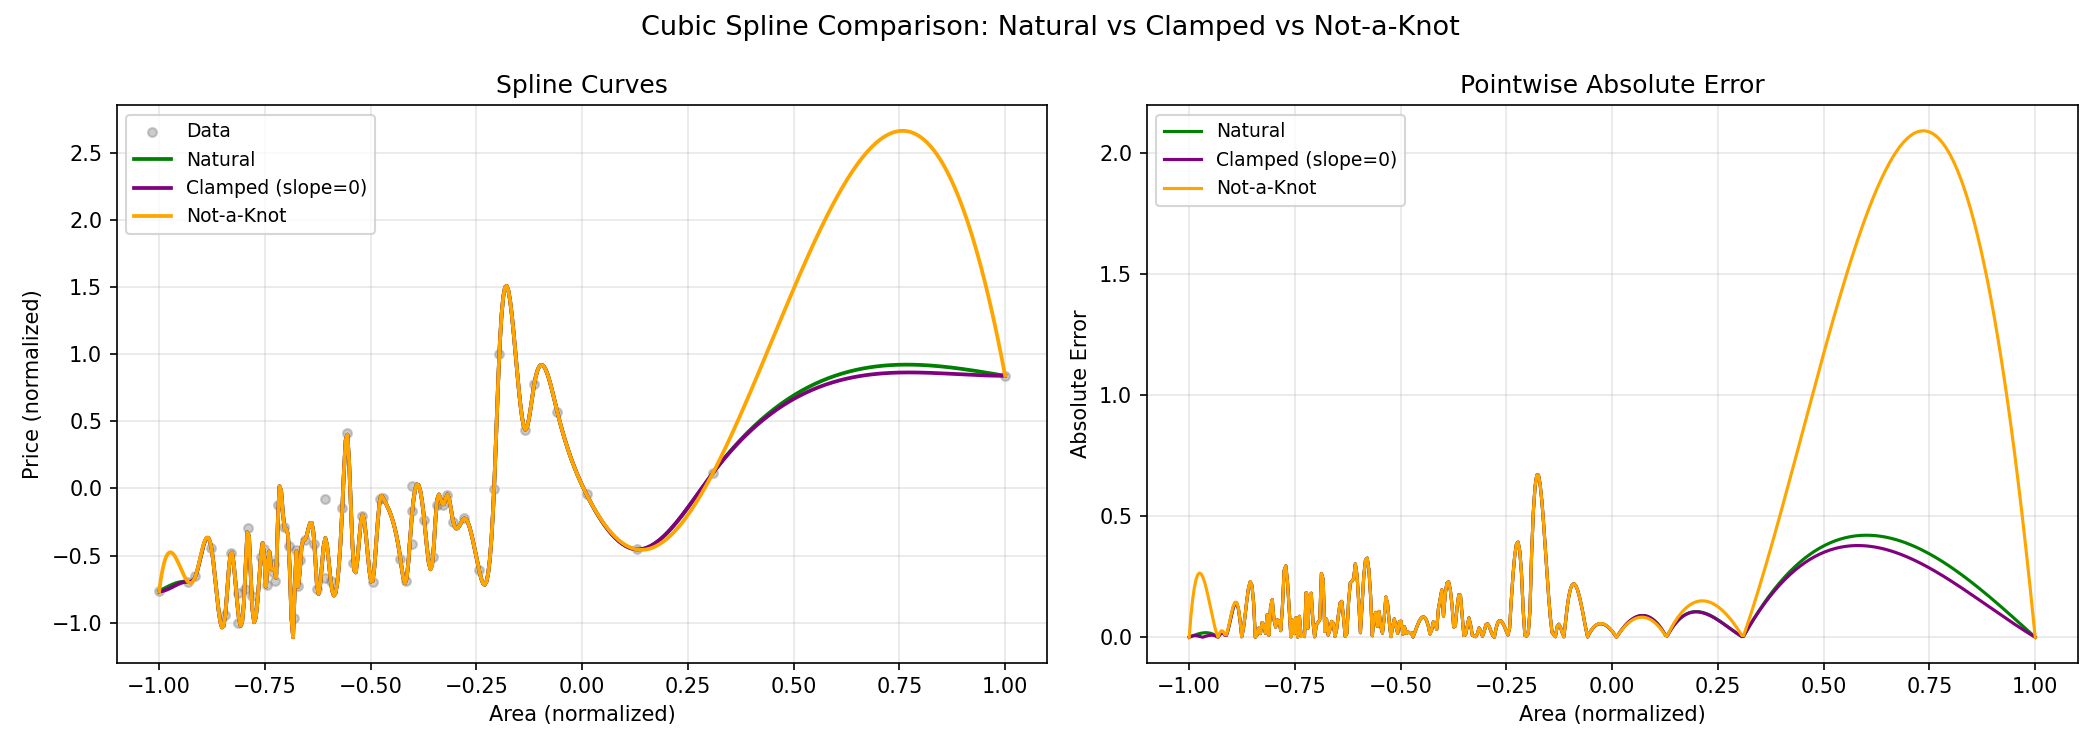
\includegraphics[width=\linewidth]{plot4_splines.png}
  \caption{%
    \textbf{Left:} Cubic spline fits under three boundary conditions.
    Natural (green) and Clamped (purple) splines are nearly identical
    and trace the data closely.  The Not-a-Knot spline (orange) deviates
    significantly near the right boundary.
    \textbf{Right:} Pointwise absolute errors, confirming the Not-a-Knot
    spline's large tail error.
  }
  \label{fig:splines}
\end{figure}

\begin{table}[h]
  \centering
  \caption{Cubic spline errors under different boundary conditions.}
  \label{tab:splines}
  \begin{tabular}{lcc}
    \toprule
    Boundary Condition & $L^\infty$ Error & $L^2$ (RMS) Error \\
    \midrule
    Natural   ($S'' = 0$ at endpoints) & 0.6695 & 0.2113 \\
    Clamped   ($S' = 0$ at endpoints)  & 0.6695 & 0.1941 \\
    Not-a-Knot                         & 2.0907 & 0.8657 \\
    \bottomrule
  \end{tabular}
\end{table}

All three splines pass through the data exactly by construction.  The
differences arise from how the two free degrees of freedom are allocated.

Natural and Clamped splines achieve identical $L^\infty$ errors of $0.6695$
and nearly identical $L^2$ errors (Table~\ref{tab:splines}).  The marginal
advantage of Clamped in $L^2$ ($0.194$ vs.\ $0.211$) reflects the fact that
imposing zero slope at the boundaries reduces extrapolative overshoot, which
the $L^2$ norm detects as a modest average improvement.

Not-a-Knot performs substantially worse ($L^\infty = 2.09$, $L^2 = 0.87$),
three times the error of Natural/Clamped.  The error plot
(Figure~\ref{fig:splines}, right) reveals the cause: a large spike in the
right half of the domain.  In datasets where the boundary region contains
few or irregular observations, the not-a-knot condition --- which enforces
continuity of the third derivative across interior knots --- can produce
undesirable oscillation.

\subsection{Experiment 4: $L^2$ vs.\ $L^\infty$ Error Comparison}

\begin{figure}[h]
  \centering
  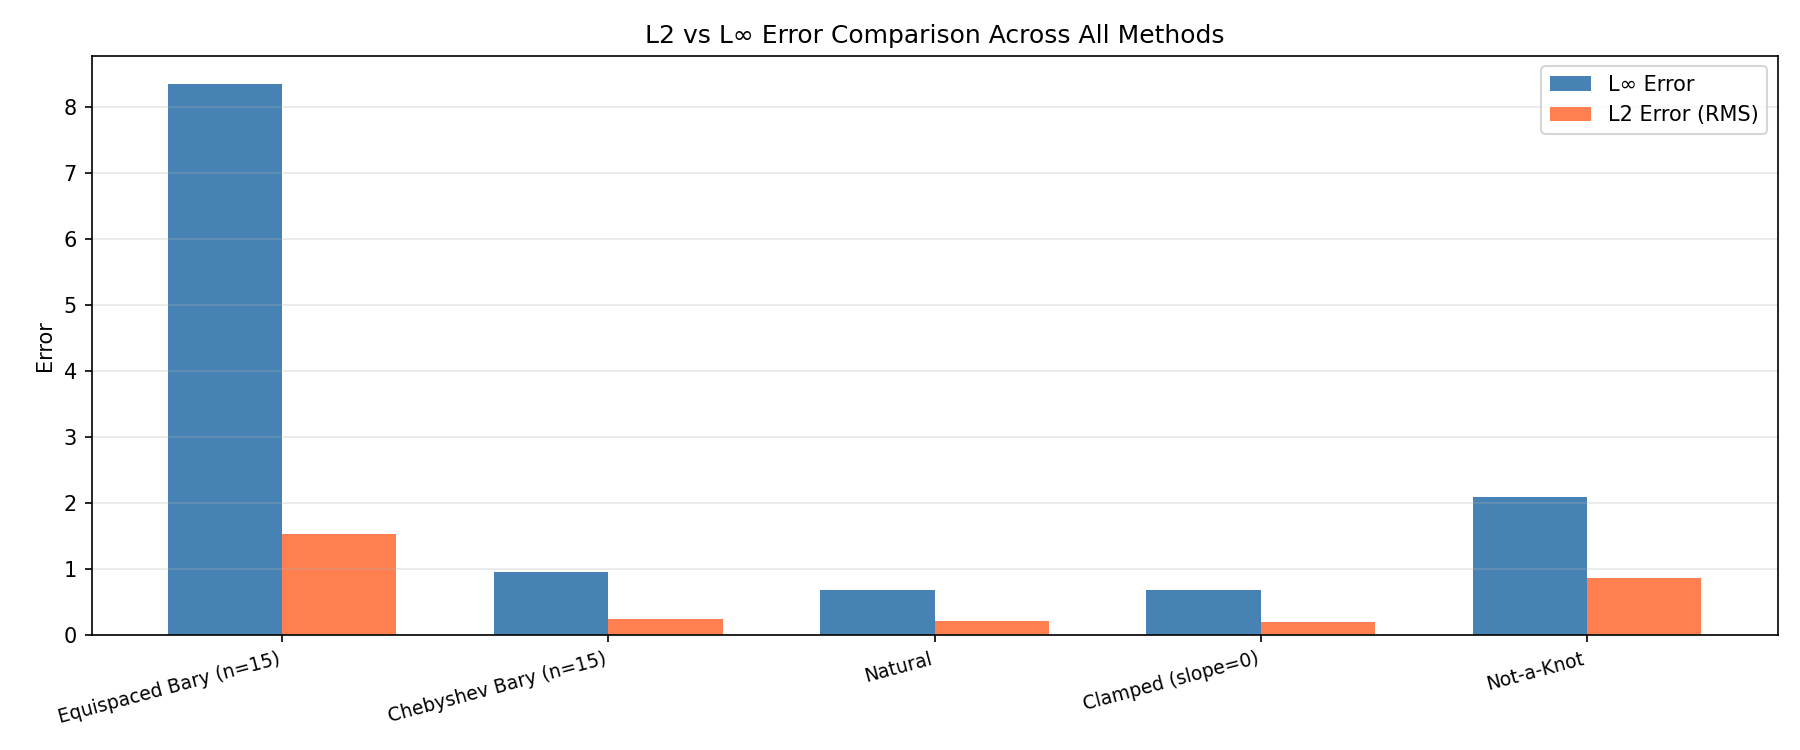
\includegraphics[width=\linewidth]{plot5_error_comparison.png}
  \caption{%
    Side-by-side $L^\infty$ (blue) and $L^2$ RMS (orange) errors across
    all five interpolation methods.  The two norms agree on ranking but
    differ dramatically in magnitude for the Equispaced method, where a
    single localized spike dominates the $L^\infty$ norm.
  }
  \label{fig:error_comparison}
\end{figure}

\begin{table}[h]
  \centering
  \caption{Full error summary across all methods ($n=15$ for barycentric).}
  \label{tab:summary}
  \begin{tabular}{lcc}
    \toprule
    Method & $L^\infty$ Error & $L^2$ (RMS) Error \\
    \midrule
    Equispaced Barycentric ($n=15$) & 8.3501 & 1.5317 \\
    Not-a-Knot Spline               & 2.0907 & 0.8657 \\
    Chebyshev Barycentric ($n=15$)  & 0.9487 & 0.2316 \\
    Natural Spline                  & 0.6695 & 0.2113 \\
    Clamped Spline                  & 0.6695 & \textbf{0.1941} \\
    \bottomrule
  \end{tabular}
\end{table}

The summary in Table~\ref{tab:summary} and Figure~\ref{fig:error_comparison}
reveals two key insights.  First, the two norms agree on the relative ranking
of methods: Clamped $\approx$ Natural $<$ Chebyshev $<$ Not-a-Knot $<$
Equispaced.  Second, the \emph{ratio} $\|e\|_\infty / \|e\|_2$ is far larger
for Equispaced ($8.35 / 1.53 \approx 5.5$) than for Chebyshev
($0.95 / 0.23 \approx 4.1$) or Natural ($0.67 / 0.21 \approx 3.2$).  This
indicates that the equispaced error is concentrated in a small region (a spike
near the boundary), while errors for the other methods are more uniformly
distributed.  The $L^\infty$ norm is thus \emph{necessary} to detect localized
Runge-type oscillations; the $L^2$ norm alone would underestimate the severity.

% =============================================================================
\section{Interpretation: Accuracy, Stability, and Conditioning}
% =============================================================================

\subsection{Accuracy}

The experimental results confirm classical theory.  The equispaced
interpolant is a \emph{divergent} sequence in $L^\infty$ for this dataset:
error grows roughly exponentially past $n = 10$.  The Chebyshev interpolant
is \emph{convergent} and stable.  Cubic splines achieve superior accuracy to
both polynomial methods at moderate $n$, because their piecewise structure
avoids the global influence of any single rogue oscillation.

\subsection{Stability and the Lebesgue Constant}

The interpolation operator $P_n : f \mapsto p_n$ is a projection.  Its
operator norm in the $L^\infty$ sense is the Lebesgue constant:
\[
  \Lambda_n = \max_{x \in [-1,1]} \sum_{k=1}^{n} |L_k(x)|,
\]
where $L_k$ are the Lagrange basis polynomials.  For equispaced nodes
$\Lambda_n$ grows exponentially, so any perturbation in the data values $y_k$
(noise, rounding) is amplified by an exponentially large factor.  For
Chebyshev nodes $\Lambda_n = O(\log n)$, giving much weaker amplification.

In practice, the plots show exactly this: the equispaced polynomial
oscillates between $-9$ and $+3$ (normalized scale) in a region where the
true data lies in $[-1, 1]$.  This is not noise amplification from floating
point error but the fundamental instability of the operator.

\subsection{Conditioning of the Interpolation Matrix}

An alternative view is through the Vandermonde matrix $V$ with
$V_{ij} = x_i^{j-1}$.  For equispaced nodes the condition number
$\kappa(V)$ grows as $O\!\left((\sqrt{3}+\sqrt{2})^{2n}\right) \approx
O(9.9^n)$, making the system exponentially ill-conditioned.  The barycentric
form avoids \emph{explicitly} constructing $V$, but the underlying ill-posedness
(the Lebesgue constant growth) persists: it is a property of the node
distribution, not the algorithm.

Chebyshev nodes approximately minimize the Lebesgue constant for a given $n$,
which is why switching from equispaced to Chebyshev nodes is sufficient to
eliminate Runge behavior entirely in this experiment.

\subsection{Spline Local Support and Smoothness}

Cubic splines avoid global oscillation because each piece $S_k$ on
$[x_k, x_{k+1}]$ depends only on nearby data.  The $C^2$ continuity
constraints propagate smoothly, and the tridiagonal system solved to find the
spline coefficients has condition number that grows only mildly with $n$.
The choice of boundary condition affects only the two outermost pieces, which
is why Natural and Clamped perform identically over most of the domain and
differ only in global $L^2$ by a few percent.

% =============================================================================
\section{Limitations and Possible Extensions}
% =============================================================================

\subsection{Limitations}

\begin{enumerate}
  \item \textbf{Univariate reduction.}  The study uses only area as a
        predictor.  Housing price is genuinely multivariate; a univariate
        interpolant captures at most the marginal relationship and conflates
        the effects of all other features into noise.

  \item \textbf{Reference function.}  The ``true'' function used for error
        evaluation is itself constructed by linear interpolation of the 60
        data points, not an analytical ground truth.  Error measurements
        therefore reflect deviation from a piecewise-linear reference, not
        from the true price-generating process.

  \item \textbf{Subsample size.}  Only 60 of 545 records are used.  Different
        subsamples could yield different qualitative conclusions about boundary
        behavior.

  \item \textbf{No generalization test.}  All errors are measured on the
        interpolation interval, not on held-out test data.  Interpolation
        accuracy on training nodes says nothing about \emph{extrapolation}
        or predictive performance.

  \item \textbf{Endpoint sensitivity.}  The dataset contains high-value
        outliers at the largest areas, and both the equispaced polynomial and
        the Not-a-Knot spline show their worst errors near these endpoints.
        Trimming or reweighting outliers might change the relative ordering of
        methods.
\end{enumerate}

\subsection{Possible Extensions}

\begin{enumerate}
  \item \textbf{Multivariate interpolation / regression splines.}  Extending
        to tensor-product or thin-plate splines would allow all ten features
        to be used simultaneously, at the cost of higher computational
        complexity.

  \item \textbf{Adaptive node selection.}  Rather than fixing nodes as
        equispaced or Chebyshev, one could select nodes adaptively based on
        local data density or estimated curvature, potentially outperforming
        both fixed distributions.

  \item \textbf{Cross-validation error.}  Replacing the in-sample error
        metric with leave-one-out or $k$-fold cross-validation would provide
        a fairer assessment of predictive accuracy.

  \item \textbf{Condition number tracking.}  Explicitly computing and plotting
        the condition number of the interpolation matrix as a function of $n$
        would provide a more rigorous theoretical corroboration of the observed
        Runge behavior.

  \item \textbf{Orthogonal polynomial regression.}  Replacing interpolation
        with least-squares fitting in the Chebyshev or Legendre polynomial
        basis would trade exact data passage for reduced sensitivity to
        outliers, a natural extension for noisy real-world data.

  \item \textbf{Trigonometric / spectral interpolation.}  For data that is
        periodic or nearly periodic (seasonal price cycles), Fourier-based
        interpolation could be explored as an alternative to polynomial methods.
\end{enumerate}

% =============================================================================
\section{Conclusion}
% =============================================================================

This study applied four families of numerical interpolation methods to a
real housing price dataset and evaluated them under two error norms.  The
central findings are:

\begin{itemize}
  \item Chebyshev barycentric interpolation reduces $L^\infty$ error by
        nearly an order of magnitude relative to equispaced nodes at the same
        polynomial degree ($n=15$), and remains stable as degree increases to
        20 --- a regime where equispaced error exceeds 280.

  \item Runge-type oscillations are unambiguously present in the equispaced
        results: the $L^\infty$ error grows exponentially past $n=10$,
        consistent with theoretical predictions based on the Lebesgue
        constant.

  \item Cubic splines with natural or clamped boundary conditions achieve the
        best overall accuracy, with $L^\infty \approx 0.67$ and $L^2 \approx
        0.19$--$0.21$, outperforming all polynomial interpolants at $n=15$.

  \item The $L^\infty$ norm is essential for detecting localized Runge
        oscillations.  The $L^2$ norm alone underestimates their severity by
        a factor of approximately 5 for the equispaced method.
\end{itemize}

These results underscore the importance of node placement and boundary
condition selection in practical interpolation, and reinforce the theoretical
superiority of Chebyshev-distributed nodes and piecewise-cubic splines over
na\"ive high-degree polynomial fits.

% =============================================================================
\begin{thebibliography}{9}

\bibitem{higham2004}
N.~J.~Higham,
\emph{The numerical stability of barycentric Lagrange interpolation},
IMA Journal of Numerical Analysis, 24(4):547--556, 2004.

\bibitem{trefethen2013}
L.~N.~Trefethen,
\emph{Approximation Theory and Approximation Practice},
SIAM, Philadelphia, 2013.

\bibitem{stoer2002}
J.~Stoer and R.~Bulirsch,
\emph{Introduction to Numerical Analysis}, 3rd ed.,
Springer, New York, 2002.

\bibitem{scipy}
P.~Virtanen et al.,
\emph{SciPy 1.0: Fundamental Algorithms for Scientific Computing in Python},
Nature Methods, 17:261--272, 2020.

\bibitem{kaggle}
Saurabhbadole,
\emph{Housing Price Data},
Kaggle, \url{https://www.kaggle.com/datasets/saurabhbadole/housing-price-data},
2023.

\end{thebibliography}

\end{document}
